\documentclass{beamer}

\usepackage{minted}

\usepackage[orientation=portrait,size=a1,scale=1.1
]{beamerposter}
\usetheme{JuelichPoster}

\setbeamertemplate{partner1}{
\includegraphics{img/cscs}}
% TODO Add HBP and/or eBrains here

\begin{document}
\begin{frame}[t, fragile]
  \frametitle{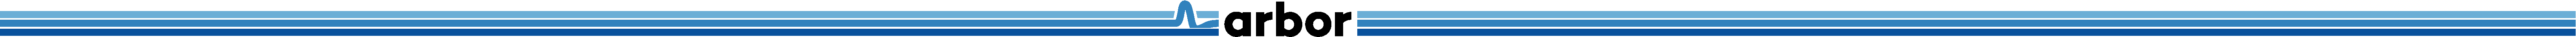
\includegraphics[width=\linewidth]{img/arbor-lines-proto-colour-full}}
  \framesubtitle{A morphologically detailed neural network simulation library for modern high performance computer architectures.\\
    \tiny{Nora Abi Akar, Ben Cumming, Stuart Yates (CSCS); Thorsten Hater, Brent Huisman, Anne Küsters (Forschungszentrum Jülich)}}

  \begin{columns}
    \begin{column}{0.65\textwidth}
      We present recent developments in Arbor, a library for the simulation of
      morphologically detailled neurons and networks thereof. Arbor places strong
      emphasis on performance, portability, and usability. It can exploit modern
      architectures based on super-scalar multi-core processors and GPU accelerators.
      We will showcase some of the features added to Arbor since the last release and
      how they can used to almost directly import single cell models from the Allen
      Brain Atlas database.
    \end{column}
    \begin{column}{0.3\textwidth}
      \begin{block}{Where to find us}
        \begin{description}
          \item[Contact] arbor-sim@fz-juelich.de
          \item[Source code] github.com/arbor-sim/arbor
          \item[Documentation] arbor.readthedocs.io
        \end{description}
      \end{block}
    \end{column}
  \end{columns}

  \begin{appendixblock}
    \begin{minipage}[c]{.48\linewidth}
      \centering
      \color{fzjblue}\rule{0.9\linewidth}{0.2\paperheight}
    \end{minipage}
    \hfill
    \begin{minipage}[c]{.48\linewidth}
      \begin{itemize}
        \item Ceaque es asitis aut quo tem ime pore recae
        \item Ceaque es asitis aut quo tem ime pore reca
        iduntiuntrepratu ritem. Nam es et ab is et estotas es repelit
        \item sit abo. Nate nos ipsum fugitaque sandaerfere doleserio
        dolor aut et dolorroreium et ipsa dolut optatur aut ad quae
        enditatusam dolorei
        \item Ceaque es asitis aut quo tem ime pore recae
        iduntiuntrepratu ritem. Nam es et ab is et estotas es repelit
      \end{itemize}
    \end{minipage}
  \end{appendixblock}

  \textbf{\structure{Running an Allen Brain Atlas Model}}\\

  We demonstrate how a model imported from the Brain Atlas database can be run using
  Arbor almost directly\cite{atlas}.\\[1.5ex]
  \begin{columns}[onlytextwidth]
    \begin{column}{.49\linewidth}
      \begin{enumerate}
        \item build the geometry by loading a SWC structure from the download
        \item assign labels to geometry
        \item build a cell description from labels and geometry
        \item parse the electro-physical properties supplied in the download and assign to regions
        \begin{enumerate}
          \item set physical properties: $T$, $V_{m}$, $R_{a}$, $C_{m}$
          \item define ion dynamics reversal potentials
        \end{enumerate}
        \item Attach to the soma's center
        \begin{enumerate}
          \item current clamp; rectangular stimulus of $150\,pA$ from $200\,ms$ to $1200\,ms$
          \item voltage probe; sampling with $200\,kHz$
          \item spike detector; triggering at $V=-40\,mV$
        \end{enumerate}
        \item convert the cell description into a runnable simulation
        \item declare that we will use a mechanism catalogue comprising
        \begin{itemize}
          \item the default mechanisms, prefixed by \texttt{default\_}
          \item the Allen DB mechanisms
        \end{itemize}
        \item Finally, run the simulation for $1400\,ms$ with time step $\Delta t = 0.0005\,ms$
      \end{enumerate}
      \includegraphics{src/arbor.pdf}
    \end{column}
    \begin{column}{.49\linewidth}
      \inputminted{python}{src/model.py}
    \end{column}
  \end{columns}
\end{frame}
\end{document}
